\subsection{Reprezentacja rozwiązania}

Reprezentacja za pomocą wektora binarnego w której jedynkę interpretujemy jako ofertę możliwą do zaakceptowania, a zero za jej definitywne odrzucenie. W szczególności, wartość 1 nie oznacza, że oferta zostanie zaakceptowana ze względu na możliwy konflikt z inną ofertą (dzięki temu zyskujemy to, że każdy osobnik w populacji koduje poprawne rozwiązanie).

Taka reprezentacja pozwoliła nam zastosować algorytm PBIL do rozwiązania tego problemu.

\subsection{Funkcja celu}
Funkcja celu analizuje wektor binarny rozwiązania od lewej do prawej, akceptując kolejne oferty których bit ustawiony jest na 1. W przypadku wykrycia sprzeczności z wcześniej zaakceptowaną ofertą jest ona pomijana.

\subsection{Rozwiązanie}
Do rozwiązania tego problemu użyliśmy algorymu PBIL.
Współczyniki uczenia, prawdopodobieństwa mutacji i zaburzenia podczas mutacji ustawiliśmy kolejno na 0.2, $\frac{1}{\text{liczba ofert}}$ i 0.1.
Liczbę iteracji ustawialiśmy na 100, a populację na 20.

\subsection{Wyniki}
Wyniki zaprezentowane są na wykresach poniżej (\ref{wyk:pbil1}, \ref{wyk:pbil2}).
Niebieską linią oznaczyliśmy najepszego osobnika dla algorytmu PBIL w danej iteracji. Zielona linia oznacza najlepszy wynik algorytmu losowego, który wybierał najlepszy element ze zbioru osobników o mocy równej liczbie elementów przetwarzanych przez algorytm PBIL.
\begin{figure}[!ht]
    \centering
    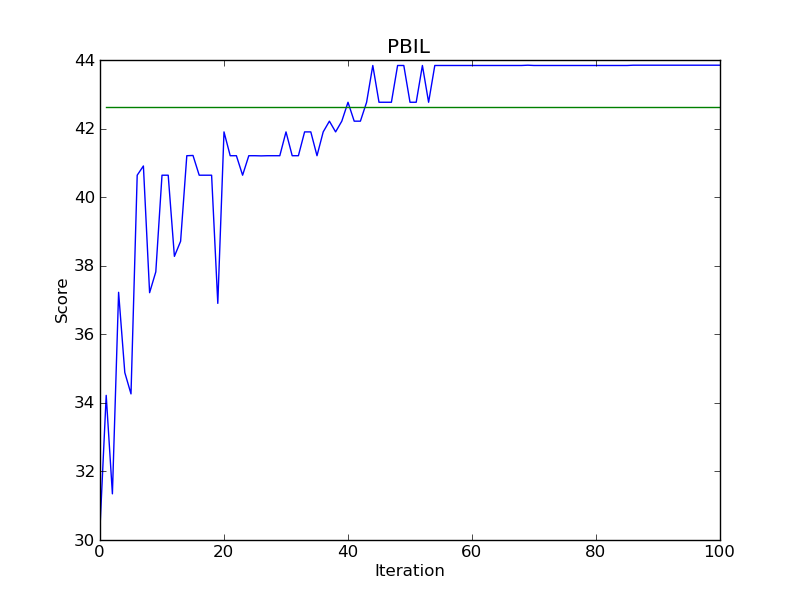
\includegraphics[width=10cm]{wykresy/matching_bids_100_goods_20_0000_txt_pbil.png}
    \caption{Wykres dla problemu 'matching' z 20 ofertami i 100 towarami.}
    \label{wyk:pbil1}
\end{figure}

\begin{figure}[!ht]
    \centering
    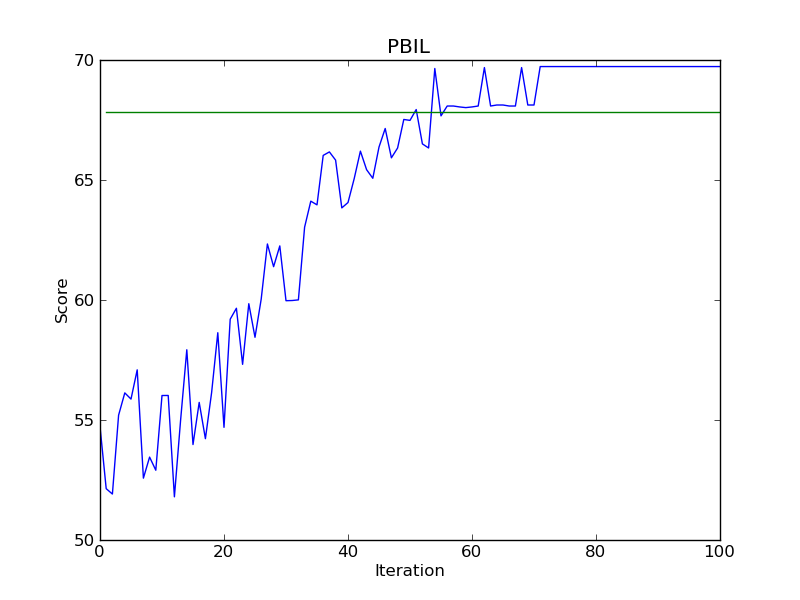
\includegraphics[width=10cm]{wykresy/matching_bids_100_goods_40_0000_txt_pbil.png}
    \caption{Wykres dla problemu 'matching' z 40 ofertami i 100 towarami.}
    \label{wyk:pbil2}
\end{figure}
